% ============================================================================
% UNIFY -- Diagram 11 (Haaniah)
% Deployment / container view: single-host Docker footprint incl. model server
% Traces to proposal v2 sec. 14 (deployment, privacy, failure behaviour),
% sec. 11.1 (local-only inference), sec. 25.5 (resource budget)
% Build: pdflatex 11_deployment.tex
% ============================================================================
\documentclass[border=12pt]{standalone}
% =============================================================================
% UNIFY -- shared TikZ style used by Haaniah's self-contained diagrams
%          (05_ingestion_sequence.tex, 06_state_machines.tex, 11_deployment.tex)
%
% Those three files each start with \documentclass{standalone} + % =============================================================================
% UNIFY -- shared TikZ style used by Haaniah's self-contained diagrams
%          (05_ingestion_sequence.tex, 06_state_machines.tex, 11_deployment.tex)
%
% Those three files each start with \documentclass{standalone} + % =============================================================================
% UNIFY -- shared TikZ style used by Haaniah's self-contained diagrams
%          (05_ingestion_sequence.tex, 06_state_machines.tex, 11_deployment.tex)
%
% Those three files each start with \documentclass{standalone} + \input{unifystyle}
% and are compiled on their own ("pdflatex <file>.tex"), unlike Mishal's and
% Abdullah's sources, which are fragments wrapped by build.sh.
%
% The original unifystyle.tex was never committed. This file was reconstructed
% so the folder is self-contained again: the palette below was sampled directly
% from the committed renders (rendered/*.png, 200 dpi), and the geometry was
% matched against them. A rebuild should reproduce the committed PDFs closely;
% if you edit a style here, re-render all three and eyeball the diff.
%
% Layout note: like unify-diagram-styles.tex, this is plain TikZ (no tikz-uml),
% so it compiles in any TeX Live.
% =============================================================================
% Times, to match the report body and the fragment diagrams
\usepackage{mathptmx}
\usepackage[T1]{fontenc}
\usepackage{tikz}
\usepackage{pgffor} % \foreach (05_ingestion_sequence lifelines)
\usetikzlibrary{arrows.meta,positioning,calc,fit,backgrounds,
                shapes.geometric,shapes.multipart,decorations.pathreplacing}

% ---- palette: exact fills sampled from the committed renders ----------------
\definecolor{extgrey}{HTML}{EDEDED}    % vendor / superseded (neutral)
\definecolor{relblue}{HTML}{CFE2F3}    % pipeline steps, fresh path
\definecolor{graphgreen}{HTML}{D9EAD3} % evidence graph / applied
\definecolor{verorange}{HTML}{FCE5CD}  % verification / findings / model
\definecolor{badred}{HTML}{F8D7DA}     % rejected / SOURCE_STALE
\definecolor{okgreen}{HTML}{DFF0D8}    % discarded / ignored / resolved
\definecolor{warnamber}{HTML}{FCE8C3}  % degraded / disputed
\definecolor{hynote}{HTML}{FFF9D6}     % side-note boxes

\tikzset{
  % ---- 05: sequence diagram --------------------------------------------------
  lane/.style={draw, fill=#1, rounded corners=2pt, inner sep=4pt,
               align=center, font=\bfseries\scriptsize},
  frame/.style={draw},                       % sdframe rectangles
  ftab/.style={draw, fill=white, font=\scriptsize, inner sep=1.5pt}, % alt A tab
  msg/.style={-{Stealth[length=2.5mm]}},     % call arrow
  ret/.style={-{Stealth[length=2.5mm]}, dashed}, % return arrow
  box/.style={draw, fill=#1, rounded corners=2pt, inner sep=4pt, align=center},
  % ---- 06: state machines ----------------------------------------------------
  st/.style={draw, fill=#1, rounded corners=2pt, inner sep=4pt,
             align=center, font=\scriptsize},
  dec/.style={diamond, aspect=1.75, draw, fill=white, font=\scriptsize,
              align=center, text width=1.5cm, inner sep=1pt},
  tr/.style={-{Stealth[length=2.2mm]}},       % state transition
  % ---- shared ----------------------------------------------------------------
  lbl/.style={font=\scriptsize, fill=white, inner sep=1pt},
  mlbl/.style={font=\scriptsize, align=center, inner sep=1pt}, % message label, sits above the arrow
  note/.style={draw, fill=hynote, font=\scriptsize, align=left,
               text width=#1, inner sep=4pt, rounded corners=2pt},
  note/.default=4.6cm,
}

% and are compiled on their own ("pdflatex <file>.tex"), unlike Mishal's and
% Abdullah's sources, which are fragments wrapped by build.sh.
%
% The original unifystyle.tex was never committed. This file was reconstructed
% so the folder is self-contained again: the palette below was sampled directly
% from the committed renders (rendered/*.png, 200 dpi), and the geometry was
% matched against them. A rebuild should reproduce the committed PDFs closely;
% if you edit a style here, re-render all three and eyeball the diff.
%
% Layout note: like unify-diagram-styles.tex, this is plain TikZ (no tikz-uml),
% so it compiles in any TeX Live.
% =============================================================================
% Times, to match the report body and the fragment diagrams
\usepackage{mathptmx}
\usepackage[T1]{fontenc}
\usepackage{tikz}
\usepackage{pgffor} % \foreach (05_ingestion_sequence lifelines)
\usetikzlibrary{arrows.meta,positioning,calc,fit,backgrounds,
                shapes.geometric,shapes.multipart,decorations.pathreplacing}

% ---- palette: exact fills sampled from the committed renders ----------------
\definecolor{extgrey}{HTML}{EDEDED}    % vendor / superseded (neutral)
\definecolor{relblue}{HTML}{CFE2F3}    % pipeline steps, fresh path
\definecolor{graphgreen}{HTML}{D9EAD3} % evidence graph / applied
\definecolor{verorange}{HTML}{FCE5CD}  % verification / findings / model
\definecolor{badred}{HTML}{F8D7DA}     % rejected / SOURCE_STALE
\definecolor{okgreen}{HTML}{DFF0D8}    % discarded / ignored / resolved
\definecolor{warnamber}{HTML}{FCE8C3}  % degraded / disputed
\definecolor{hynote}{HTML}{FFF9D6}     % side-note boxes

\tikzset{
  % ---- 05: sequence diagram --------------------------------------------------
  lane/.style={draw, fill=#1, rounded corners=2pt, inner sep=4pt,
               align=center, font=\bfseries\scriptsize},
  frame/.style={draw},                       % sdframe rectangles
  ftab/.style={draw, fill=white, font=\scriptsize, inner sep=1.5pt}, % alt A tab
  msg/.style={-{Stealth[length=2.5mm]}},     % call arrow
  ret/.style={-{Stealth[length=2.5mm]}, dashed}, % return arrow
  box/.style={draw, fill=#1, rounded corners=2pt, inner sep=4pt, align=center},
  % ---- 06: state machines ----------------------------------------------------
  st/.style={draw, fill=#1, rounded corners=2pt, inner sep=4pt,
             align=center, font=\scriptsize},
  dec/.style={diamond, aspect=1.75, draw, fill=white, font=\scriptsize,
              align=center, text width=1.5cm, inner sep=1pt},
  tr/.style={-{Stealth[length=2.2mm]}},       % state transition
  % ---- shared ----------------------------------------------------------------
  lbl/.style={font=\scriptsize, fill=white, inner sep=1pt},
  mlbl/.style={font=\scriptsize, align=center, inner sep=1pt}, % message label, sits above the arrow
  note/.style={draw, fill=hynote, font=\scriptsize, align=left,
               text width=#1, inner sep=4pt, rounded corners=2pt},
  note/.default=4.6cm,
}

% and are compiled on their own ("pdflatex <file>.tex"), unlike Mishal's and
% Abdullah's sources, which are fragments wrapped by build.sh.
%
% The original unifystyle.tex was never committed. This file was reconstructed
% so the folder is self-contained again: the palette below was sampled directly
% from the committed renders (rendered/*.png, 200 dpi), and the geometry was
% matched against them. A rebuild should reproduce the committed PDFs closely;
% if you edit a style here, re-render all three and eyeball the diff.
%
% Layout note: like unify-diagram-styles.tex, this is plain TikZ (no tikz-uml),
% so it compiles in any TeX Live.
% =============================================================================
% Times, to match the report body and the fragment diagrams
\usepackage{mathptmx}
\usepackage[T1]{fontenc}
\usepackage{tikz}
\usepackage{pgffor} % \foreach (05_ingestion_sequence lifelines)
\usetikzlibrary{arrows.meta,positioning,calc,fit,backgrounds,
                shapes.geometric,shapes.multipart,decorations.pathreplacing}

% ---- palette: exact fills sampled from the committed renders ----------------
\definecolor{extgrey}{HTML}{EDEDED}    % vendor / superseded (neutral)
\definecolor{relblue}{HTML}{CFE2F3}    % pipeline steps, fresh path
\definecolor{graphgreen}{HTML}{D9EAD3} % evidence graph / applied
\definecolor{verorange}{HTML}{FCE5CD}  % verification / findings / model
\definecolor{badred}{HTML}{F8D7DA}     % rejected / SOURCE_STALE
\definecolor{okgreen}{HTML}{DFF0D8}    % discarded / ignored / resolved
\definecolor{warnamber}{HTML}{FCE8C3}  % degraded / disputed
\definecolor{hynote}{HTML}{FFF9D6}     % side-note boxes

\tikzset{
  % ---- 05: sequence diagram --------------------------------------------------
  lane/.style={draw, fill=#1, rounded corners=2pt, inner sep=4pt,
               align=center, font=\bfseries\scriptsize},
  frame/.style={draw},                       % sdframe rectangles
  ftab/.style={draw, fill=white, font=\scriptsize, inner sep=1.5pt}, % alt A tab
  msg/.style={-{Stealth[length=2.5mm]}},     % call arrow
  ret/.style={-{Stealth[length=2.5mm]}, dashed}, % return arrow
  box/.style={draw, fill=#1, rounded corners=2pt, inner sep=4pt, align=center},
  % ---- 06: state machines ----------------------------------------------------
  st/.style={draw, fill=#1, rounded corners=2pt, inner sep=4pt,
             align=center, font=\scriptsize},
  dec/.style={diamond, aspect=1.75, draw, fill=white, font=\scriptsize,
              align=center, text width=1.5cm, inner sep=1pt},
  tr/.style={-{Stealth[length=2.2mm]}},       % state transition
  % ---- shared ----------------------------------------------------------------
  lbl/.style={font=\scriptsize, fill=white, inner sep=1pt},
  mlbl/.style={font=\scriptsize, align=center, inner sep=1pt}, % message label, sits above the arrow
  note/.style={draw, fill=hynote, font=\scriptsize, align=left,
               text width=#1, inner sep=4pt, rounded corners=2pt},
  note/.default=4.6cm,
}


\begin{document}
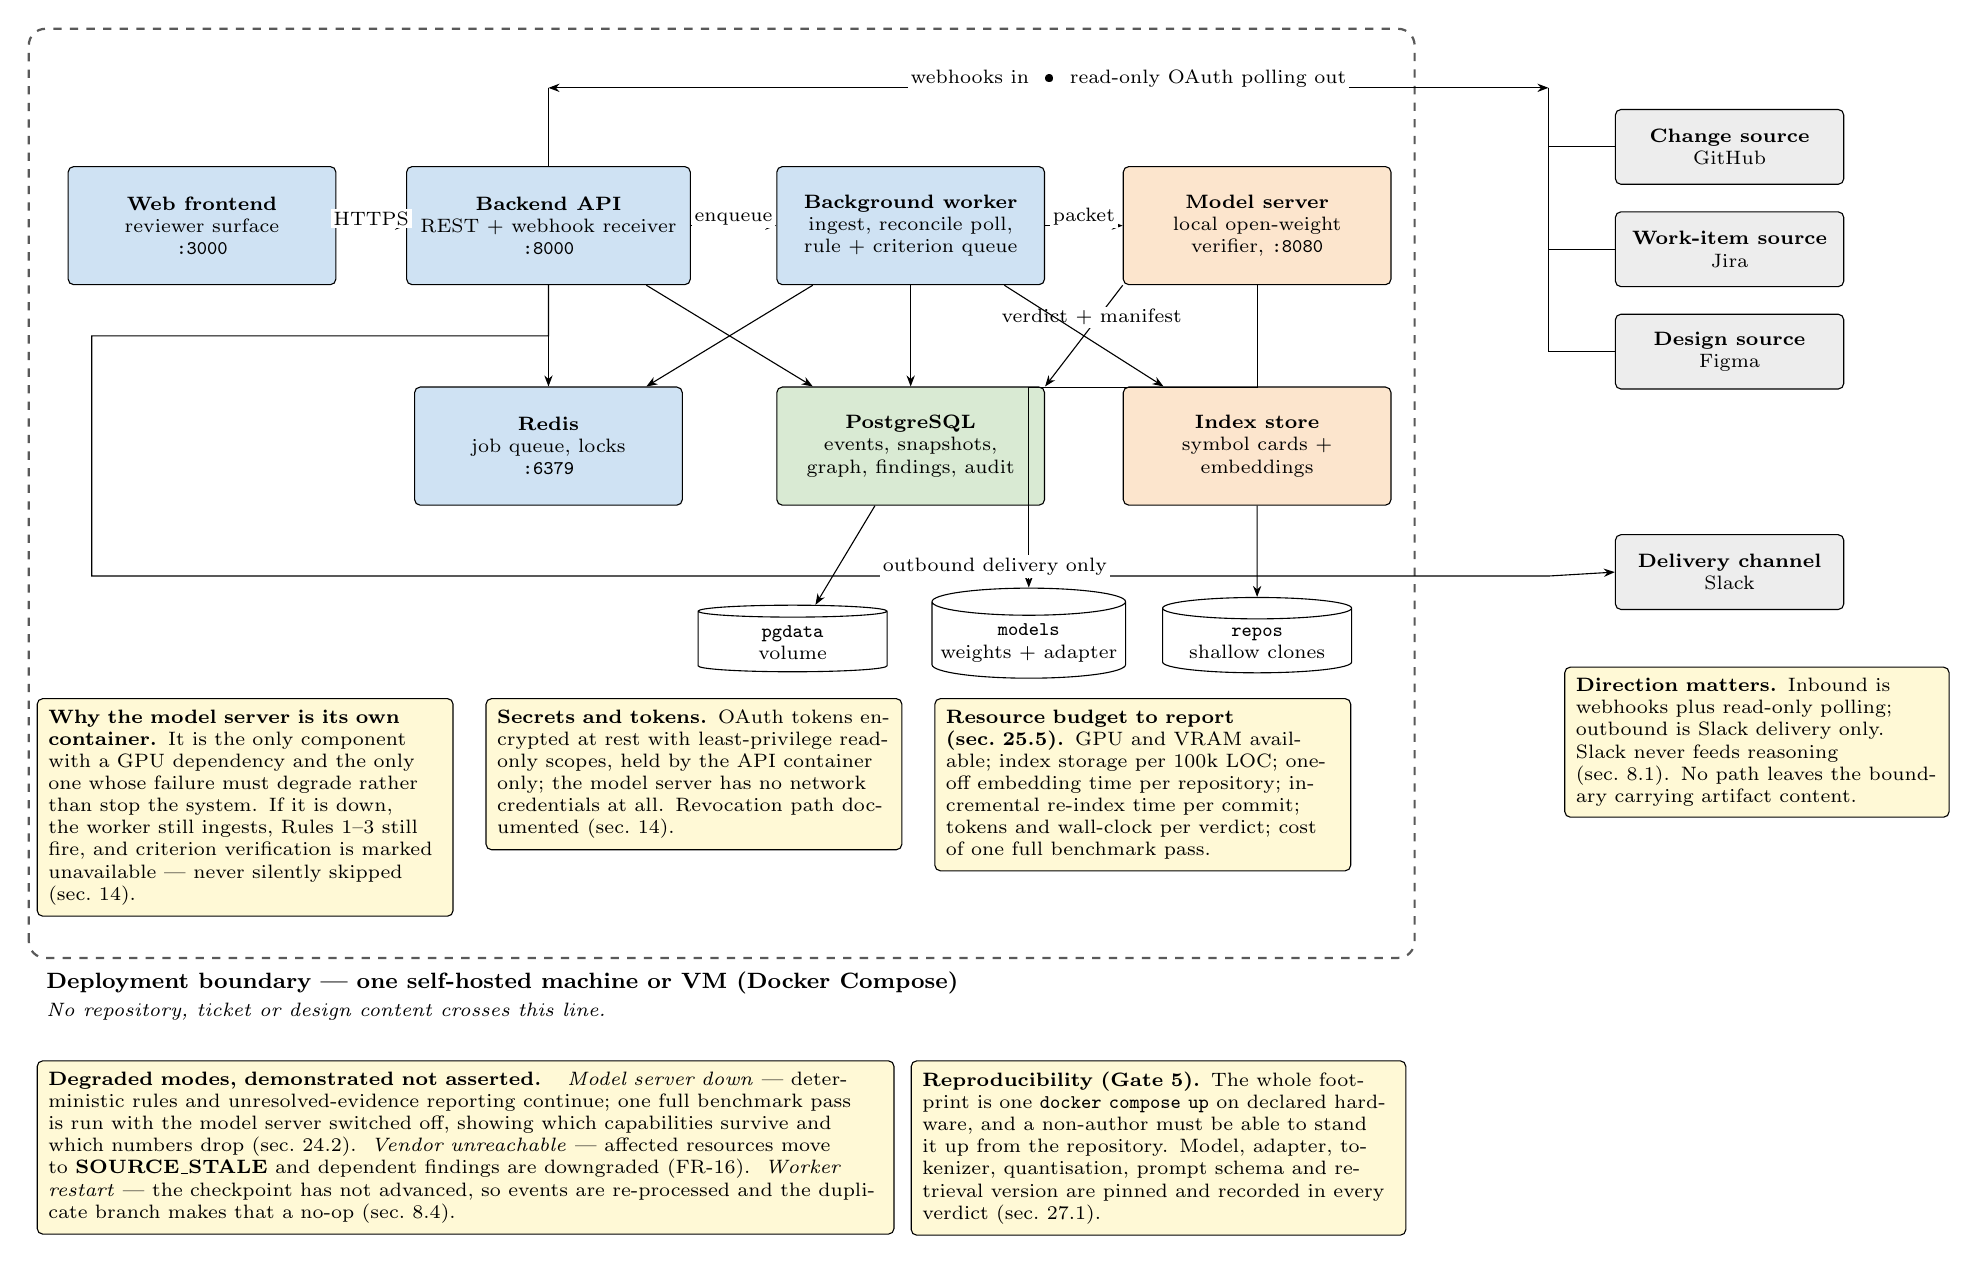
\begin{tikzpicture}[x=1cm,y=1cm]

\tikzset{
  ctr/.style={draw,fill=#1,rounded corners=2pt,inner sep=5pt,font=\scriptsize,align=center,
              minimum width=3.4cm,minimum height=1.5cm},
  vol/.style={draw,fill=white,cylinder,shape border rotate=90,aspect=0.14,inner sep=3pt,
              font=\scriptsize,align=center,minimum width=2.4cm},
  ext/.style={draw,fill=extgrey,rounded corners=2pt,inner sep=4pt,font=\scriptsize,align=center,
              minimum width=2.9cm,minimum height=0.95cm},
  flow/.style={-{Stealth[length=4pt]},thin,font=\scriptsize},
}

% ===================== host boundary ====================================
\draw[draw=black!65,dashed,thick,rounded corners=6pt] (-0.6,-9.9) rectangle (17.0,1.9);
\node[anchor=north west,font=\footnotesize\bfseries] at (-0.5,-9.95)
  {Deployment boundary --- one self-hosted machine or VM (Docker Compose)};
\node[anchor=north west,font=\scriptsize\itshape] at (-0.5,-10.35)
  {No repository, ticket or design content crosses this line.};

% ===================== containers =======================================
\node[ctr=relblue]   (web)  at ( 1.6,-0.6) {\textbf{Web frontend}\\reviewer surface\\\texttt{:3000}};
\node[ctr=relblue]   (api)  at ( 6.0,-0.6) {\textbf{Backend API}\\REST + webhook receiver\\\texttt{:8000}};
\node[ctr=relblue]   (wrk)  at (10.6,-0.6) {\textbf{Background worker}\\ingest, reconcile poll,\\rule + criterion queue};
\node[ctr=verorange] (mdl)  at (15.0,-0.6) {\textbf{Model server}\\local open-weight\\verifier, \texttt{:8080}};

\node[ctr=relblue]   (redis)at ( 6.0,-3.4) {\textbf{Redis}\\job queue, locks\\\texttt{:6379}};
\node[ctr=graphgreen](pg)   at (10.6,-3.4) {\textbf{PostgreSQL}\\events, snapshots,\\graph, findings, audit};
\node[ctr=verorange] (idx)  at (15.0,-3.4) {\textbf{Index store}\\symbol cards +\\embeddings};

\node[vol] (vpg)  at ( 9.1,-5.9) {\texttt{pgdata}\\volume};
\node[vol] (vwt)  at (12.1,-5.9) {\texttt{models}\\weights + adapter};
\node[vol] (vrepo)at (15.0,-5.9) {\texttt{repos}\\shallow clones};

\draw[flow] (web) -- node[lbl,above=-1pt]{HTTPS} (api);
\draw[flow] (api) -- node[lbl,above=-1pt]{enqueue} (wrk);
\draw[flow] (api) -- (redis);
\draw[flow] (wrk) -- (redis);
\draw[flow] (api) -- (pg);
\draw[flow] (wrk) -- (pg);
\draw[flow] (wrk) -- node[lbl,above=-1pt]{packet} (mdl);
\draw[flow] (mdl.south west) -- node[lbl,above=-1pt,pos=.4]{verdict + manifest} (pg.north east);
\draw[flow] (wrk) -- (idx);
\draw[flow] (pg)  -- (vpg);
\draw[flow] (mdl.south) -- ++(0,-1.3) -| (vwt);
\draw[flow] (idx) -- (vrepo);

% ===================== external systems =================================
\node[ext] (gh)  at (21.0, 0.4) {\textbf{Change source}\\GitHub};
\node[ext] (jr)  at (21.0,-0.9) {\textbf{Work-item source}\\Jira};
\node[ext] (fg)  at (21.0,-2.2) {\textbf{Design source}\\Figma};
\node[ext] (sl)  at (21.0,-5.0) {\textbf{Delivery channel}\\Slack};

% bundled inbound channel, routed above the container row
\draw[thin] (gh.west) -- (18.7, 0.4);
\draw[thin] (jr.west) -- (18.7,-0.9);
\draw[thin] (fg.west) -- (18.7,-2.2);
\draw[thin] (18.7,-2.2) -- (18.7,1.15);
\draw[{Stealth[length=4pt]}-{Stealth[length=4pt]},thin] (18.7,1.15)
      -- node[lbl,above=-1pt,pos=.42]{webhooks in \ \textbullet\ \ read-only OAuth polling out} (6.0,1.15);
\draw[thin] (6.0,1.15) -- (api.north);

% outbound delivery only
\draw[flow] (api.south) -- (6.0,-2.0) -- (0.2,-2.0) -- (0.2,-5.05) -- node[lbl,above=-1pt,pos=.62]{outbound delivery only} (18.7,-5.05) -- (sl.west);

\node[note=4.6cm,anchor=north west] at (18.9,-6.2)
  {\textbf{Direction matters.} Inbound is webhooks plus read-only polling;
   outbound is Slack delivery only. Slack never feeds reasoning
   (sec.~8.1). No path leaves the boundary carrying artifact content.};

% ===================== notes ============================================
\node[note=5.0cm,anchor=north west] at (-0.5,-6.6)
  {\textbf{Why the model server is its own container.}
   It is the only component with a GPU dependency and the only one whose
   failure must degrade rather than stop the system. If it is down, the
   worker still ingests, Rules~1--3 still fire, and criterion verification
   is marked unavailable --- never silently skipped (sec.~14).};

\node[note=5.0cm,anchor=north west] at (5.2,-6.6)
  {\textbf{Secrets and tokens.} OAuth tokens encrypted at rest with
   least-privilege read-only scopes, held by the API container only; the
   model server has no network credentials at all. Revocation path
   documented (sec.~14).};

\node[note=5.0cm,anchor=north west] at (10.9,-6.6)
  {\textbf{Resource budget to report (sec.~25.5).}
   GPU and VRAM available; index storage per 100k LOC; one-off embedding
   time per repository; incremental re-index time per commit; tokens and
   wall-clock per verdict; cost of one full benchmark pass.};

\node[note=10.6cm,anchor=north west] at (-0.5,-11.2)
  {\textbf{Degraded modes, demonstrated not asserted.}
   \ \ \emph{Model server down} --- deterministic rules and unresolved-evidence
   reporting continue; one full benchmark pass is run with the model server
   switched off, showing which capabilities survive and which numbers drop
   (sec.~24.2).\ \
   \emph{Vendor unreachable} --- affected resources move to \textbf{SOURCE\_STALE}
   and dependent findings are downgraded (FR-16).\ \
   \emph{Worker restart} --- the checkpoint has not advanced, so events are
   re-processed and the duplicate branch makes that a no-op (sec.~8.4).};

\node[note=6.0cm,anchor=north west] at (10.6,-11.2)
  {\textbf{Reproducibility (Gate 5).} The whole footprint is one
   \texttt{docker compose up} on declared hardware, and a non-author must be
   able to stand it up from the repository. Model, adapter, tokenizer,
   quantisation, prompt schema and retrieval version are pinned and recorded
   in every verdict (sec.~27.1).};

\end{tikzpicture}
\end{document}
